\documentclass[12pt]{article}
\usepackage[english]{babel}
\usepackage[utf8x]{inputenc}
\usepackage[font=small,labelfont=bf]{caption}
\usepackage{amsmath}
\usepackage{graphicx}
\usepackage[colorinlistoftodos]{todonotes}
\usepackage{tabularx} % in the preamble

\begin{document}
	
	\begin{titlepage}
		
		\newcommand{\HRule}{\rule{\linewidth}{0.5mm}} % Defines a new command for the horizontal lines, change thickness here
		
		\center % Center everything on the page
		
		%----------------------------------------------------------------------------------------
		%	HEADING SECTIONS
		%----------------------------------------------------------------------------------------
		
		\textsc{\LARGE Central Washington University}\\[1.5cm] % Name of your university/college
		\textsc{\Large CS 471 OPTIMIZATION}\\[0.5cm] % Major heading such as course name
		\textsc{\large Spring 2019}\\[0.5cm] % Minor heading such as course title
		
		%----------------------------------------------------------------------------------------
		%	TITLE SECTION
		%----------------------------------------------------------------------------------------
		
		\HRule \\[0.4cm]
		{ \huge \bfseries Project 4 Report}\\[0.4cm] % Title of your document
		\HRule \\[1.5cm]
		
		%----------------------------------------------------------------------------------------
		%	AUTHOR SECTION
		%----------------------------------------------------------------------------------------
		
		\begin{minipage}{0.4\textwidth}
			\begin{flushleft} \large
				\emph{Author:}\\
				Hermann \textsc{Yepdjio} % Your name
			\end{flushleft}
		\end{minipage}
		~
		\begin{minipage}{0.4\textwidth}
			\begin{flushright} \large
				\emph{Supervisor:} \\
				Dr. Donald \textsc{Davendra} % Supervisor's Name
			\end{flushright}
		\end{minipage}\\[1cm]
		
		% If you don't want a supervisor, uncomment the two lines below and remove the section above
		%\Large \emph{Author:}\\
		%John \textsc{Smith}\\[3cm] % Your name
		
		%----------------------------------------------------------------------------------------
		%	DATE SECTION
		%----------------------------------------------------------------------------------------
		
		{\large \today}\\ % Date, change the \today to a set date if you want to be precise
		
		%----------------------------------------------------------------------------------------
		%	LOGO SECTION
		%----------------------------------------------------------------------------------------
		
		
\includegraphics[width=12cm]{CWU-Logo.png}\\[.5cm] % Include a department/university logo - this will require the graphicx package
		
		%----------------------------------------------------------------------------------------
		
		\vfill % Fill the rest of the page with whitespace
		
	\end{titlepage}
	\newpage
	\tableofcontents
	\newpage
	
	
	
	\section{Introduction}
	Project 4 was about optimizing 18 standard benchmark functions namely Schwefel, De Jong 1, Rosenbrock's Saddle, Rastrigin, Griewangk, Sine Envelope Sine Wave, Stretch V Sine Wave, Ackley One, Ackley Two, Egg Holder, Rana, Pathological, Michalewicz, Master's Cosine Wave, Quartic, Levy, Step and Alpine. For this purpose, 3 optimization algorithms were to be implemented then applied to those functions. Those algorithms are: Particle Swarm Optimization (PSO), Firefly Algorithm (FA) and Harmony Search (HS) . After they have been implemented, those algorithms were run on each of the 18 benchmark functions using randomly generated data. Statistics for each algorithm were computed and stored in a tabular format and they will be discussed then analyzed later on in this report. However, in order to observe how the fitness of each objective function evolves across iterations, the first experiment was picked for each algorithm and its results were plotted. Those plots are also analyzed later on in this report.
	
		
	\section{Results}
	
		\subsection{ Particle Swarm Optimization}
		
			\subsubsection{Values used for the parameters}
				The PSO program was  run using  the following values:
				\begin{itemize}
					\item dimension: 30
					\item population size: 500
					\item number of iterations: 500
					\item number of experiments: 30
					\item c1: 0.3
					\item c2: 0.8
					\item k: 0.00001(for First De Jong, Rosenbrock and Quartic) and 0.1 (for the other functions) 
				\end{itemize}
			After experimenting with different values for c1, c2 and k, it appeared that only varying k could make a significant impact on the outcome of the objective functions. Therefore, 0.00001 was chosen for First De Jong, Rosenbrock and Quartic and 0.1 was chosen for the rest as they seemed to work pretty well for their respective functions.
		
			\subsubsection{Statistics}
				% latex table generated in R 3.5.3 by xtable 1.8-4 package
				% Mon May 20 00:33:17 2019
				\begin{table}[ht]
						\caption{Statistics for PSO (30 experiments)}
						\centering
						\scalebox{0.9}{
							\begin{tabular}{lllllll}
								\hline
								& {\textbf{Average}} & {\textbf{Std\_Dev}} & {\textbf{Range}} & {\textbf{Median}} & {\textbf{Avg\_Time}} & {\textbf{Avg \#calls$\backslash$exp}} \\ 
								\hline
								{\textit{f1 Schwefel}} & 0.20 & 0.51 & 2.65 & 0.05 & 396.60 & 250500 \\ 
								{\textit{f2 De Jong 1}} & 0.00 & 0.00 & 0.00 & 0.00 & 261.70 & 250500 \\ 
								{\textit{f3 Rosenbrock}} & 4.31 & 5.66 & 24.22 & 1.80 & 380.10 & 250500 \\ 
								{\textit{f4 Rastrigin}} & 220176.30 & 47554.73 & 208458.00 & 226013.00 & 441.23 & 250500 \\ 
								{\textit{f5 Griewangk}} & 1.01 & 0.00 & 0.00 & 1.01 & 499.87 & 250500 \\ 
								{\textit{f6 Sine Envelope}} & -20.49 & 0.65 & 2.41 & -20.57 & 741.33 & 250500 \\ 
								{\textit{f7 Stretch V Sine}} & 10.15 & 0.00 & 0.00 & 10.15 & 747.03 & 250500 \\ 
								{\textit{f8 Ackley One}} & 5.89 & 3.69 & 12.01 & 6.69 & 633.63 & 250500 \\ 
								{\textit{f9 Ackley Two}} & 0.32 & 0.35 & 1.30 & 0.25 & 881.27 & 250500 \\ 
								{\textit{f10 Egg Holder}} & -4880.27 & 458.96 & 1927.40 & -4899.37 & 629.73 & 250500 \\ 
								{\textit{f11 Rana}} & -3310.65 & 302.34 & 1235.29 & -3313.05 & 926.03 & 250500 \\ 
								{\textit{f12 Pathological}} & 0.00 & 0.00 & 0.00 & 0.00 & 721.10 & 250500 \\ 
								{\textit{f13 Michalewicz}} & -7.88 & 0.55 & 2.32 & -7.90 & 1105.03 & 250500 \\ 
								{\textit{f14 Masters’ Cosine}} & -15.67 & 0.00 & 0.00 & -15.67 & 693.50 & 250500 \\ 
								{\textit{f15 Quartic}} & 0.00 & 0.00 & 0.01 & 0.00 & 681.30 & 250500 \\ 
								{\textit{f16 Levy}} & 0.00 & 0.00 & 0.00 & 0.00 & 721.77 & 250500 \\ 
								{\textit{f17 Step}} & 7.39 & 0.11 & 0.40 & 7.36 & 271.03 & 250500 \\ 
								{\textit{f18 Alpine}} & 0.03 & 0.03 & 0.15 & 0.02 & 376.23 & 250500 \\ 
								\hline
							\end{tabular}
						}
					\end{table}
				
			\subsubsection{Statistics analysis}
			
				As table 1 above shows, PSO produced pretty good results for all the objective functions. Those results are even better (except for the Rastrigin function (220176.30 vs -89999.93) ) than those produced by the Differential Evolution Algorithm in the previous assignment.
			\subsubsection{plots}
				\begin{minipage}{0.6\linewidth}
					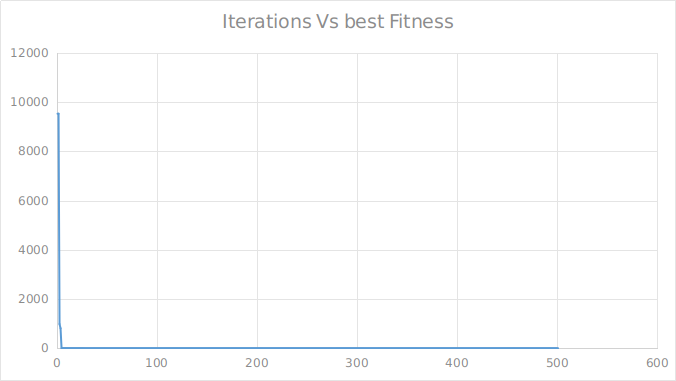
\includegraphics[width=\linewidth]{1.png}
					\captionof{figure}{Schwefel (Experiment \#1)}
				\end{minipage}
				\hfill
				\begin{minipage}{0.6\linewidth}
					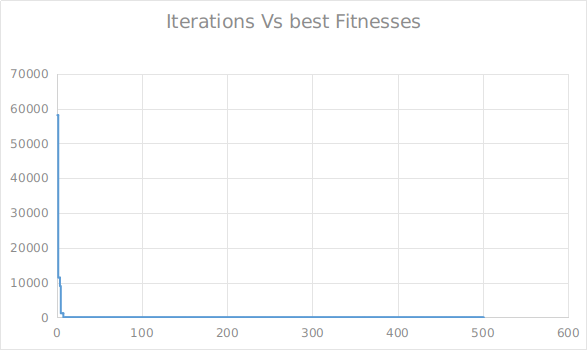
\includegraphics[width=\linewidth]{2.png}
					\captionof{figure}{De Jong 1 (Experiment \#1)}
				\end{minipage}
				\begin{minipage}{0.6\linewidth}
					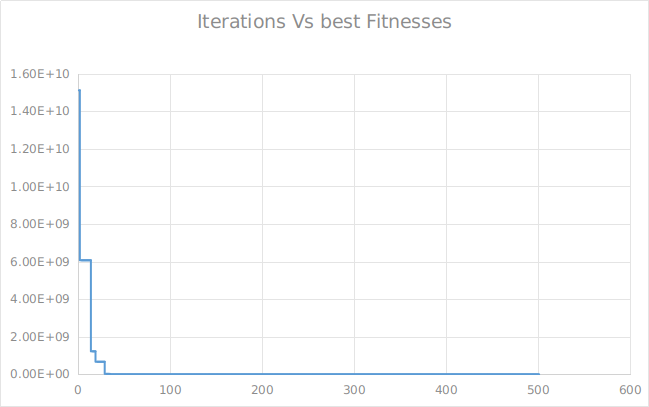
\includegraphics[width=\linewidth]{3.png}
					\captionof{figure}{Rosenbrock (Experiment \#1)}
				\end{minipage}
				\hfill
				\begin{minipage}{0.6\linewidth}
					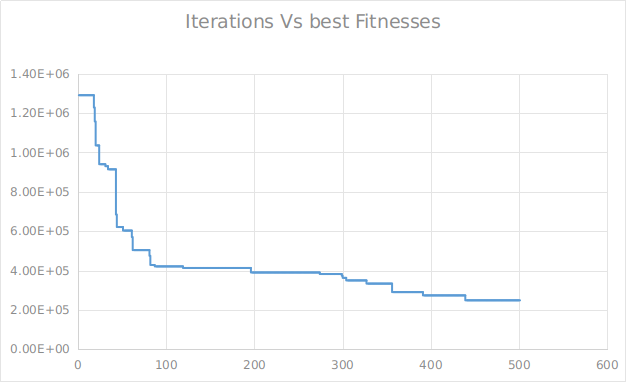
\includegraphics[width=\linewidth]{4.png}
					\captionof{figure}{Rastrigin (Experiment \#1)}
				\end{minipage}
				\begin{minipage}{0.6\linewidth}
					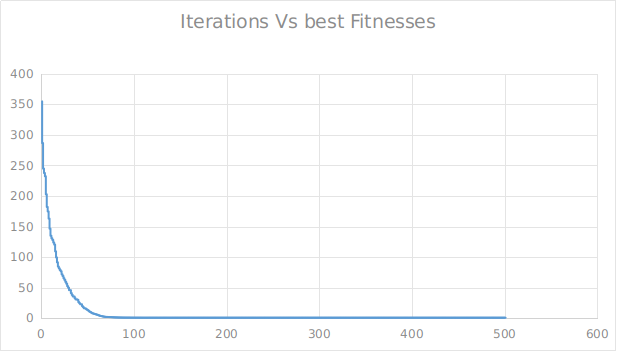
\includegraphics[width=\linewidth]{5.png}
					\captionof{figure}{Griewangk (Experiment \#1)}
				\end{minipage}
				\hfill
				\begin{minipage}{0.6\linewidth}
					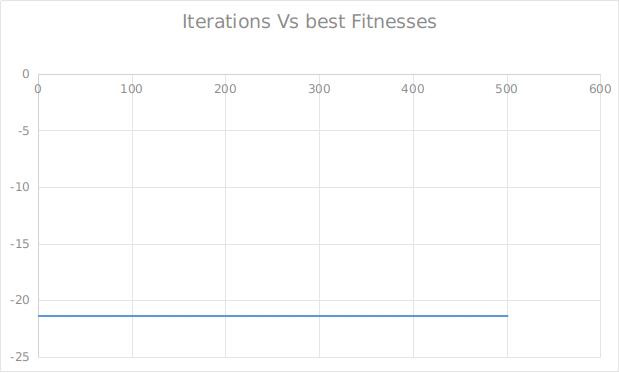
\includegraphics[width=\linewidth]{6.png}
					\captionof{figure}{Sine Envelope (Experiment \#1)}
				\end{minipage}
				\begin{minipage}{0.6\linewidth}
					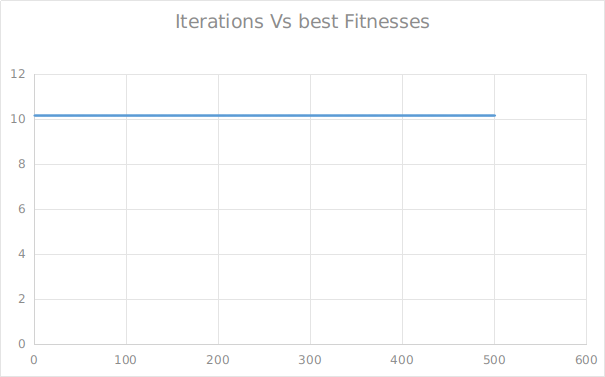
\includegraphics[width=\linewidth]{7.png}
					\captionof{figure}{Stretch V Sine (Experiment \#1)}
				\end{minipage}
				\hfill
				\begin{minipage}{0.6\linewidth}
					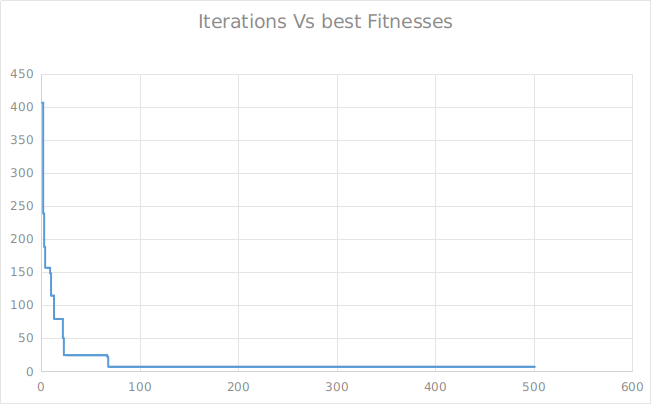
\includegraphics[width=\linewidth]{8.png}
					\captionof{figure}{Ackley One (Experiment \#1)}
				\end{minipage}
				\begin{minipage}{0.6\linewidth}
					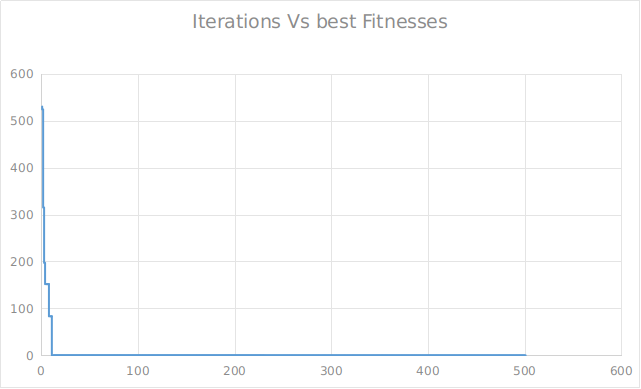
\includegraphics[width=\linewidth]{9.png}
					\captionof{figure}{Ackley Two (Experiment \#1)}
				\end{minipage}
				\hfill
				\begin{minipage}{0.6\linewidth}
					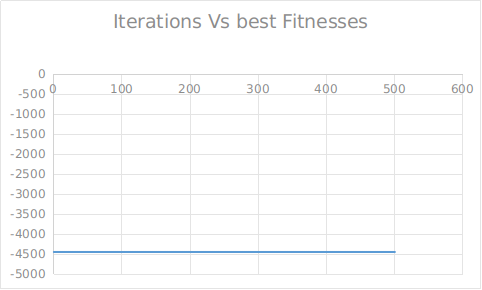
\includegraphics[width=\linewidth]{10.png}
					\captionof{figure}{Egg Holder (Experiment \#1)}
				\end{minipage}
				\begin{minipage}{0.6\linewidth}
					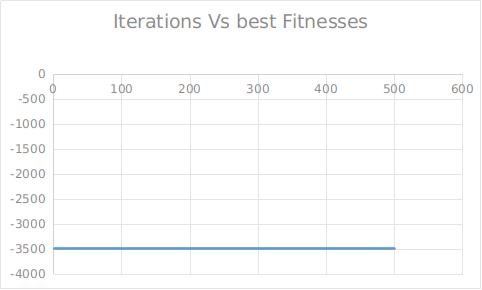
\includegraphics[width=\linewidth]{11.png}
					\captionof{figure}{Rana (Experiment \#1)}
				\end{minipage}
				\hfill
				\begin{minipage}{0.6\linewidth}
					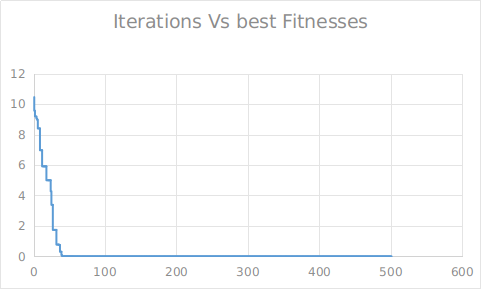
\includegraphics[width=\linewidth]{12.png}
					\captionof{figure}{Pathological (Experiment \#1)}
				\end{minipage}
				\begin{minipage}{0.6\linewidth}
					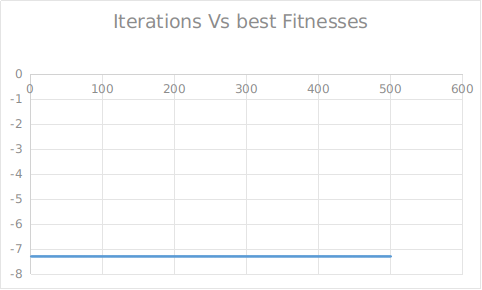
\includegraphics[width=\linewidth]{13.png}
					\captionof{figure}{Michalewicz (Experiment \#1)}
				\end{minipage}
				\hfill
				\begin{minipage}{0.6\linewidth}
					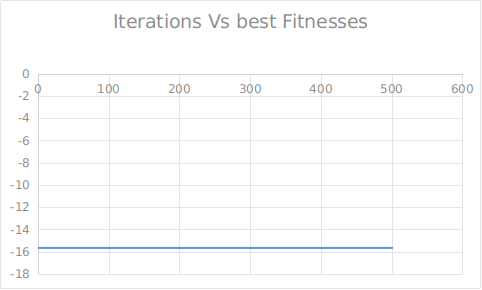
\includegraphics[width=\linewidth]{14.png}
					\captionof{figure}{Masters’ Cosine (Experiment \#1)}
				\end{minipage}
				\begin{minipage}{0.6\linewidth}
					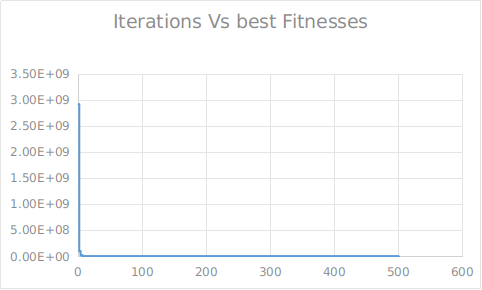
\includegraphics[width=\linewidth]{15.png}
					\captionof{figure}{Quartic (Experiment \#1)}
				\end{minipage}
				\hfill
				\begin{minipage}{0.6\linewidth}
					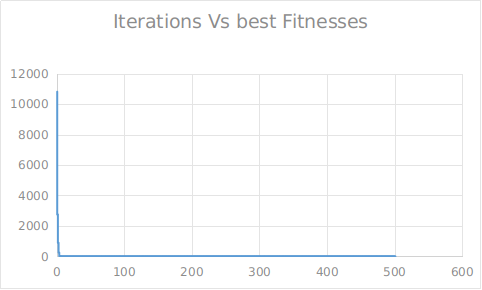
\includegraphics[width=\linewidth]{16.png}
					\captionof{figure}{Levy (Experiment \#1)}
				\end{minipage}
				\begin{minipage}{0.6\linewidth}
					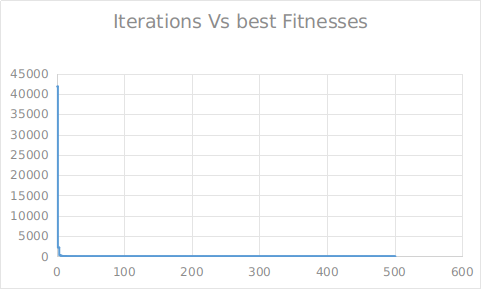
\includegraphics[width=\linewidth]{17.png}
					\captionof{figure}{Step (Experiment \#1)}
				\end{minipage}
				\hfill
				\begin{minipage}{0.6\linewidth}
					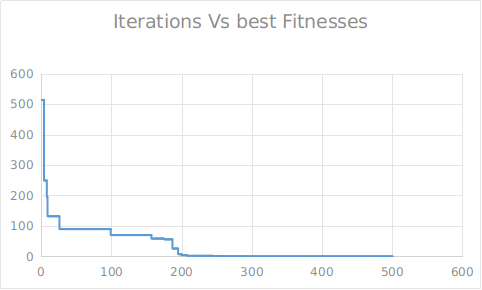
\includegraphics[width=\linewidth]{18.png}
					\captionof{figure}{Alpine (Experiment \#1)}
				\end{minipage}
				\subsubsection{Plots analysis}
					When looking at the figures above, we can see that PSO improves the quality of the solutions as it goes through iterations. The reason to this improvement is that after each iteration, the less fitted particles try to adjust their speeds in order to get closer to the best fitted ones. However, Figures 6, 7,10, 11, 13 and 14 corresponding to functions Sine Envelope, Stretch V Sine, Egg Holder, Rana, Michalewicz and Master's Cosine respectively also show that PSO does not work well for all the functions. In this case, the best solutions do not improve nor they deteriorate. 
				\subsubsection{Stagnation iterations}
	
					% latex table generated in R 3.5.3 by xtable 1.8-4 package
					% Mon May 20 00:55:44 2019
					\begin{table}[ht]
						\caption{Iteration at which population stagnates (0 means no stagnation observed)}
						\centering
							\scalebox{0.7}{
								\begin{tabular}{lllllllllllllllllll}
									\hline
									& {\textbf{f1}} & {\textbf{f2}} & {\textbf{f3}} & {\textbf{f4}} & {\textbf{f5}} & {\textbf{f6}} & {\textbf{f7}} & {\textbf{f8}} & {\textbf{f9}} & {\textbf{f10}} & {\textbf{f11}} & {\textbf{f12}} & {\textbf{f13}} & {\textbf{f14}} & {\textbf{f15}} & {\textbf{f16}} & {\textbf{f17}} & {\textbf{f18}} \\ 
									\hline
									{\textit{iter 1}} &   0 &   0 &  26 &   0 &   0 &   0 &   0 &   0 &   0 &   0 &   0 &   0 &   0 &   0 &   0 &   0 &   0 &   0 \\ 
									{\textit{iter 2}} &   0 &   0 &  12 &   0 &   0 &   0 &   0 &   0 &   0 &   0 &   0 &   0 &   0 &   0 &   0 &   0 &   0 &   0 \\ 
									{\textit{fiter 3}} &   0 &   0 &  13 &   0 &   0 &   0 &   0 &   0 &   0 &   0 &   0 &   0 &   0 &   0 &   0 &   0 &   0 &   0 \\ 
									{\textit{iter 4}} &   0 &   0 &  14 &   0 &   0 &   0 &   0 &   0 &   0 &   0 &   0 &   0 &   0 &   0 &   0 &   0 &   0 &   0 \\ 
									{\textit{iter 5}} &   0 &   0 &   8 &   0 &   0 &   0 &   0 &   0 &   0 &   0 &   0 &   0 &   0 &   0 &   0 &   0 &   0 &   0 \\ 
									{\textit{iter 6}} &   0 &   0 &  35 &   0 &   0 &   0 &   0 &   0 &   0 &   0 &   0 &   0 &   0 &   0 &   0 &   0 &   5 &   0 \\ 
									{\textit{iter 7}} &   0 &   0 &   0 &   0 &   0 &   0 &   0 &   0 &   0 &   0 &   0 &   0 &   0 &   0 &   0 &   0 &   0 &   0 \\ 
									{\textit{iter 8}} &   0 &   0 &   0 &   0 &   0 &   0 &   0 &   0 &   0 &   0 &   0 &   0 &   0 &   0 &   0 &   0 &   0 &   0 \\ 
									{\textit{iter 9}} &   0 &   0 &  18 &   0 &   0 &   0 &   0 &   0 &   0 &   0 &   0 &   0 &   0 &   0 &   0 &   0 &   0 &   0 \\ 
									{\textit{iter 10}} &   0 &   0 &  29 &   0 &   0 &   0 &   0 &   0 &   0 &   0 &   0 &   0 &   0 &   0 &   0 &   0 &   0 &   0 \\ 
									{\textit{iter 11}} &   0 &   0 &  16 &   0 &   0 &   0 &   0 &   0 &   0 &   0 &   0 &   0 &   0 &   0 &   2 &   0 &   0 &   0 \\ 
									{\textit{iter 12}} &   0 &   0 &  37 &   0 &   0 &   0 &   0 &   0 &   0 &   0 &   0 &   0 &   0 &   0 &   0 &   0 &   0 &   0 \\ 
									{\textit{iter 13}} &   0 &   0 &  24 &   0 &   0 &   0 &   0 &   0 &   0 &   0 &   0 &   0 &   0 &   0 &   0 &   0 &   0 &   0 \\ 
									{\textit{iter 14}} &   0 &   0 &  11 &   0 &   0 &   0 &   0 &   0 &   0 &   0 &   0 &   0 &   0 &   0 &   0 &   0 &   0 &   0 \\ 
									{\textit{iter 15}} &   0 &   0 &   3 &   0 &   0 &   0 &   0 &   0 &   0 &   0 &   0 &   0 &   0 &   0 &   0 &   0 &   0 &   0 \\ 
									{\textit{iter 16}} &   0 &   0 &   2 &   0 &   0 &   0 &   0 &   0 &   0 &   0 &   0 &   0 &   0 &   0 &   0 &   0 &   0 &   0 \\ 
									{\textit{iter 17}} &   0 &   0 &   9 &   0 &   0 &   0 &   0 &   0 &   0 &   0 &   0 &   0 &   0 &   0 &   0 &   0 &   0 &   0 \\ 
									{\textit{iter 18}} &   0 &   0 &   7 &   0 &   0 &   0 &   0 &   0 &   0 &   0 &   0 &   0 &   0 &   0 &   0 &   0 &   0 &   0 \\ 
									{\textit{iter 19}} &   0 &   0 &   5 &   0 &   0 &   0 &   0 &   0 &   0 &   0 &   0 &   0 &   0 &   0 &   0 &   0 &   0 &   0 \\ 
									{\textit{iter 20}} &   0 &   0 &  46 &   0 &   0 &   0 &   0 &   0 &   0 &   0 &   0 &   0 &   0 &   0 &   0 &   0 &   0 &   0 \\ 
									{\textit{iter 21}} &   0 &   0 &   5 &   0 &   0 &   0 &   0 &   0 &   0 &   0 &   0 &   0 &   0 &   0 &   0 &   0 &   0 &   0 \\ 
									{\textit{iter 22}} &   0 &   5 &   0 &   0 &   0 &   0 &   0 &   0 &   0 &   0 &   0 &   0 &   0 &   0 &   0 &   0 &   0 &   0 \\ 
									{\textit{iter 23}} &   0 &   0 &   3 &   0 &   0 &   0 &   0 &   0 &   0 &   0 &   0 &   0 &   0 &   0 &   0 &   0 &   9 &   0 \\ 
									{\textit{iter 24}} &   0 &   0 &   5 &   0 &   0 &   0 &   0 &   0 &   0 &   0 &   0 &   0 &   0 &   0 &   0 &   0 &   0 &   0 \\ 
									{\textit{iter 25}} &   0 &   0 &  23 &   0 &   0 &   0 &   0 &   0 &   0 &   0 &   0 &   0 &   0 &   0 &   0 &   0 &   0 &   0 \\ 
									{\textit{iter 26}} &   0 &   3 &  24 &   0 &   0 &   0 &   0 &   0 &   0 &   0 &   0 &   0 &   0 &   0 &   0 &   0 &   0 &   0 \\ 
									{\textit{iter 27}} &   0 &   0 &  26 &   0 &   0 &   0 &   0 &   0 &   0 &   0 &   0 &   0 &   0 &   0 &   0 &   0 &   0 &   0 \\ 
									{\textit{iter 28}} &   0 &   4 &  11 &   0 &   0 &   0 &   0 &   0 &   0 &   0 &   0 &   0 &   0 &   0 &   0 &   0 &   0 &   0 \\ 
									{\textit{iter 29}} &   0 &   0 &  16 &   0 &   0 &   0 &   0 &   0 &   0 &   0 &   0 &   0 &   0 &   0 &   2 &   0 &   3 &   0 \\ 
									{\textit{iter 30}} &   0 &   0 &   8 &   0 &   0 &   0 &   0 &   0 &   0 &   0 &   0 &   0 &   0 &   0 &   3 &   0 &   0 &   0 \\ 
									\hline
								\end{tabular}
							}
					\end{table}
		
			\subsection{Firefly Algorithm}
				\subsubsection{Values used for the parameters}
					The Firefly Algorithm was  run using  the following values:
					\begin{itemize}
						\item dimension: 30
						\item population size: 500
						\item number of generations: 500
						\item number of experiments: 30
						\item $\gamma$: 1
						\item $\beta_0$: 0.2
						\item $\alpha$: 0.5
					\end{itemize}
				
					Experiments were performed while varying the values for $\gamma$, $\beta_0$ and $\alpha$ but all the results looked similar.
					
				\subsubsection{Statistics}
				\newpage
					% latex table generated in R 3.5.3 by xtable 1.8-4 package
					% Mon May 20 00:30:38 2019
					\begin{table}
							\caption{Statistics for FA (30 experiments)}
							\centering
							\scalebox{0.9}{
								\begin{tabular}{lllllll}
									\hline
									& {\textbf{Average}} & {\textbf{Std\_Dev}} & {\textbf{Range}} & {\textbf{Median}} & {\textbf{Avg\_Time}} & {\textbf{Avg \#calls$\backslash$exp}} \\ 
									\hline
									{\textit{f1 Schwefel}} & 9190.78 & 237.84 & 985.20 & 9232.69 & 167793.93 & 4.93E+07 \\ 
									{\textit{f2 De Jong 1}} & 1.67 & 0.16 & 0.67 & 1.69 & 100650.17 & 3.43E+07 \\ 
									{\textit{f3 Rosenbrock}} & 131.14 & 9.40 & 35.02 & 132.95 & 167647.10 & 4.96E+07 \\ 
									{\textit{f4 Rastrigin}} & 25.91 & 55.34 & 282.34 & 7.84 & 211564.90 & 5.73E+07 \\ 
									{\textit{f5 Griewangk}} & 1.00 & 0.00 & 0.00 & 1.00 & 36595.37 & 9.13E+06 \\ 
									{\textit{f6 Sine Envelope}} & -20.22 & 0.70 & 2.57 & -20.15 & 303557.50 & 6.16E+07 \\ 
									{\textit{f7 Stretch V Sine}} & 10.15 & 0.00 & 0.00 & 10.15 & 371.17 & 500 \\ 
									{\textit{f8 Ackley One}} & 3.77 & 1.59 & 6.36 & 3.81 & 264987.13 & 5.96E+07 \\ 
									{\textit{f9 Ackley Two}} & 62.15 & 3.26 & 15.05 & 63.11 & 341409.83 & 6.17E+07 \\ 
									{\textit{f10 Egg Holder}} & -5092.90 & 578.42 & 1992.42 & -5196.45 & 219777.37 & 5.29E+07 \\ 
									{\textit{f11 Rana}} & -3399.74 & 408.34 & 1885.43 & -3429.27 & 307177.87 & 5.71E+07 \\ 
									{\textit{f12 Pathological}} & 0.00 & 0.00 & 0.00 & 0.00 & 293725.87 & 5.76E+07 \\ 
									{\textit{f13 Michalewicz}} & -8.02 & 0.59 & 2.32 & -7.85 & 387429.70 & 6.16E+07 \\ 
									{\textit{f14 Masters’ Cosine}} & -15.67 & 0.00 & 0.00 & -15.67 & 366.80 & 500 \\ 
									{\textit{f15 Quartic}} & 2.67 & 0.57 & 2.15 & 2.65 & 212631.63 & 4.71E+07 \\ 
									{\textit{f16 Levy}} & 0.59 & 0.07 & 0.33 & 0.59 & 299312.63 & 6.13E+07 \\ 
									{\textit{f17 Step}} & 14.45 & 0.50 & 1.97 & 14.58 & 101594.60 & 3.41E+07 \\ 
									{\textit{f18 Alpine}} & 2.16 & 0.17 & 0.58 & 2.21 & 204291.83 & 6.13E+07 \\ 
									\hline
								\end{tabular}
							}
					\end{table}
				
				\subsubsection{Statistics Analysis}
				
					As table 3 above shows, the Firefly Algorithm performed a little less better than PSO for most of the objective functions. However, for some functions such as Rastrigin, it produced really good results compared to the corresponding results for PSO(25.91 vs 220176.30). Table 3 also shows that, FA takes a lot of time to process compared to all the other algorithms seen so far.
				\subsubsection{plots}
				
					\begin{minipage}{0.6\linewidth}
						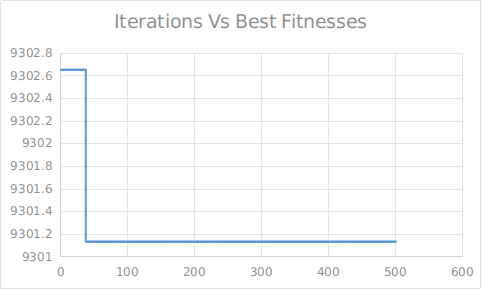
\includegraphics[width=\linewidth]{19.png}
						\captionof{figure}{Schwefel (Experiment \#1)}
					\end{minipage}
					\hfill
					\begin{minipage}{0.6\linewidth}
						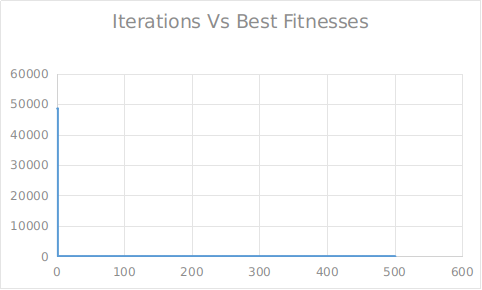
\includegraphics[width=\linewidth]{20.png}
						\captionof{figure}{De Jong 1 (Experiment \#1)}
					\end{minipage}
					\begin{minipage}{0.6\linewidth}
						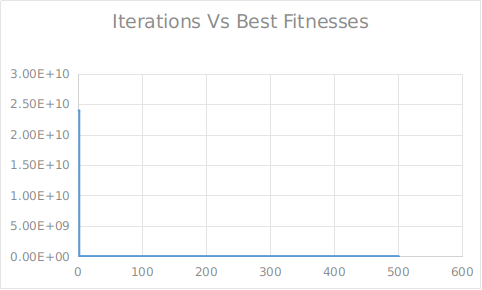
\includegraphics[width=\linewidth]{21.png}
						\captionof{figure}{Rosenbrock (Experiment \#1)}
					\end{minipage}
					\hfill
					\begin{minipage}{0.6\linewidth}
						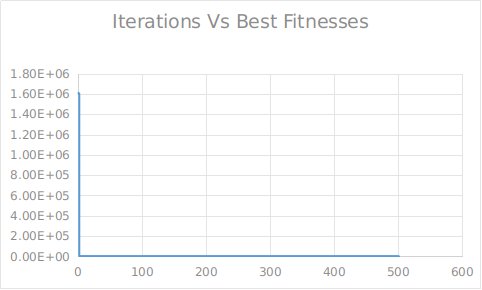
\includegraphics[width=\linewidth]{22.png}
						\captionof{figure}{Rastrigin (Experiment \#1)}
					\end{minipage}
					\begin{minipage}{0.6\linewidth}
						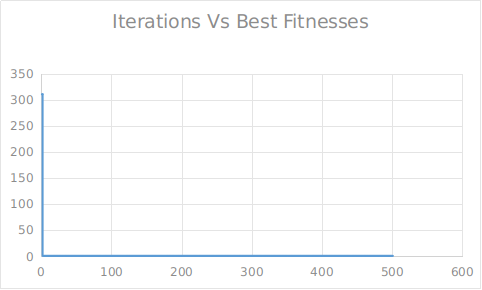
\includegraphics[width=\linewidth]{23.png}
						\captionof{figure}{Griewangk (Experiment \#1)}
					\end{minipage}
					\hfill
					\begin{minipage}{0.6\linewidth}
						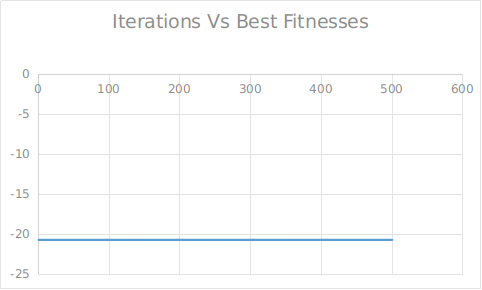
\includegraphics[width=\linewidth]{24.png}
						\captionof{figure}{Sine Envelope (Experiment \#1)}
					\end{minipage}
					\begin{minipage}{0.6\linewidth}
						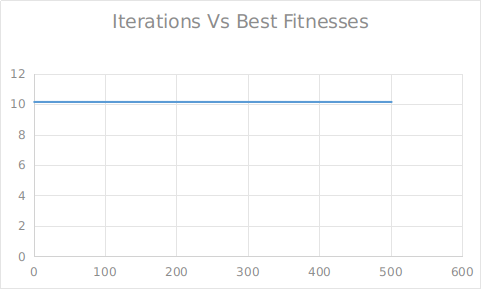
\includegraphics[width=\linewidth]{25.png}
						\captionof{figure}{Stretch V Sine (Experiment \#1)}
					\end{minipage}
					\hfill
					\begin{minipage}{0.6\linewidth}
						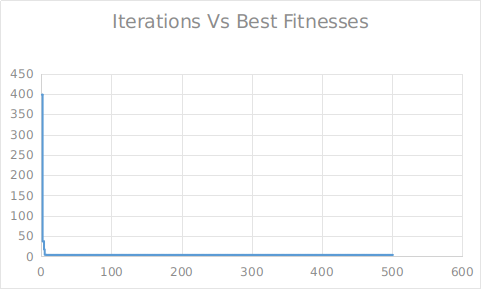
\includegraphics[width=\linewidth]{26.png}
						\captionof{figure}{Ackley One (Experiment \#1)}
					\end{minipage}
					\begin{minipage}{0.6\linewidth}
						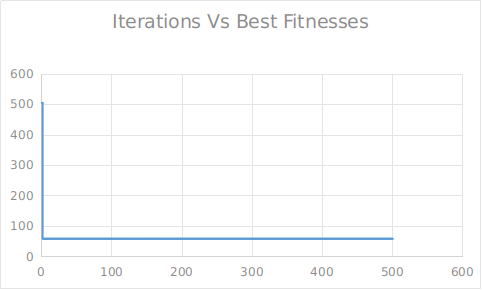
\includegraphics[width=\linewidth]{27.png}
						\captionof{figure}{Ackley Two (Experiment \#1)}
					\end{minipage}
					\hfill
					\begin{minipage}{0.6\linewidth}
						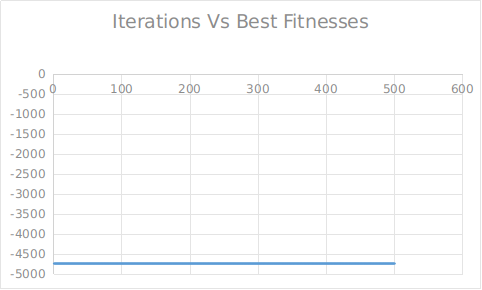
\includegraphics[width=\linewidth]{28.png}
						\captionof{figure}{Egg Holder (Experiment \#1)}
					\end{minipage}
					\begin{minipage}{0.6\linewidth}
						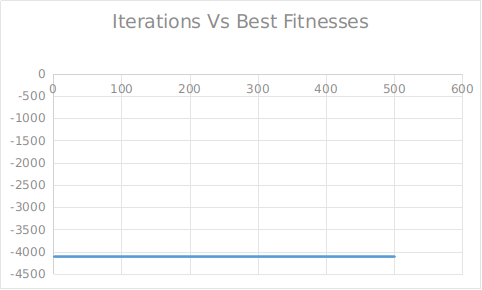
\includegraphics[width=\linewidth]{29.png}
						\captionof{figure}{Rana (Experiment \#1)}
					\end{minipage}
					\hfill
					\begin{minipage}{0.6\linewidth}
						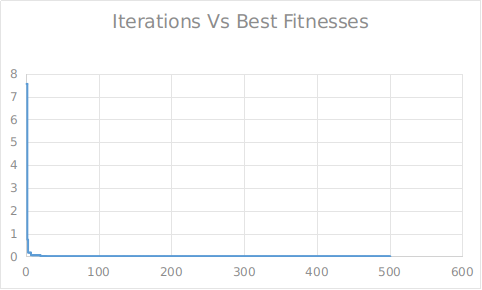
\includegraphics[width=\linewidth]{30.png}
						\captionof{figure}{Pathological (Experiment \#1)}
					\end{minipage}
					\begin{minipage}{0.6\linewidth}
						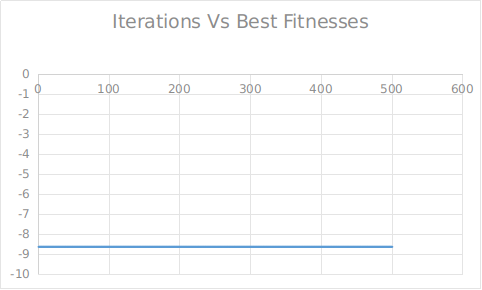
\includegraphics[width=\linewidth]{31.png}
						\captionof{figure}{Michalewicz (Experiment \#1)}
					\end{minipage}
					\hfill
					\begin{minipage}{0.6\linewidth}
						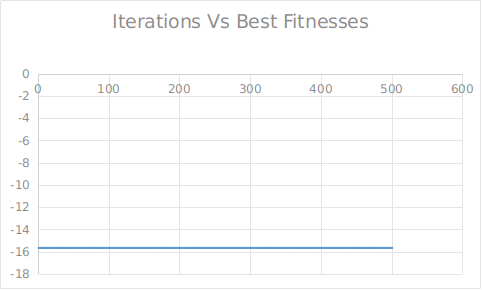
\includegraphics[width=\linewidth]{32.png}
						\captionof{figure}{Masters’ Cosine (Experiment \#1)}
					\end{minipage}
					\begin{minipage}{0.6\linewidth}
						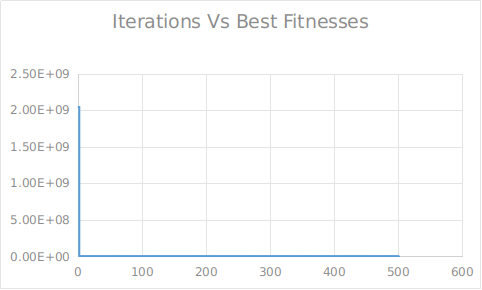
\includegraphics[width=\linewidth]{33.png}
						\captionof{figure}{Quartic (Experiment \#1)}
					\end{minipage}
					\hfill
					\begin{minipage}{0.6\linewidth}
						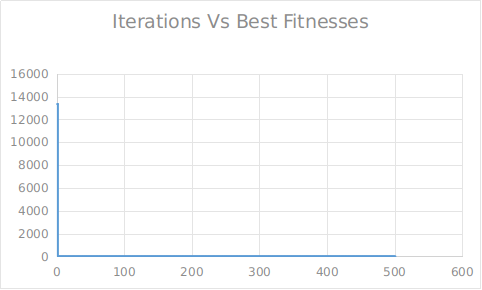
\includegraphics[width=\linewidth]{34.png}
						\captionof{figure}{Levy (Experiment \#1)}
					\end{minipage}
					\begin{minipage}{0.6\linewidth}
						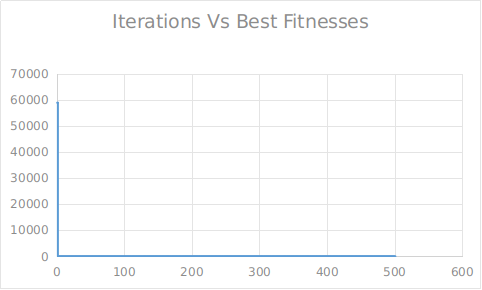
\includegraphics[width=\linewidth]{35.png}
						\captionof{figure}{Step (Experiment \#1)}
					\end{minipage}
					\hfill
					\begin{minipage}{0.6\linewidth}
						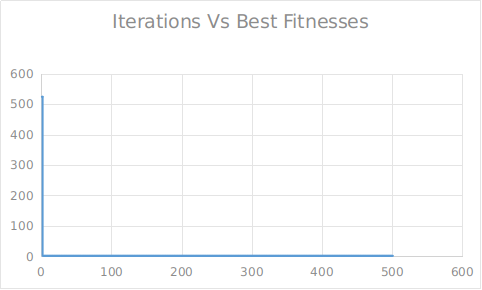
\includegraphics[width=\linewidth]{36.png}
						\captionof{figure}{Alpine (Experiment \#1)}
					\end{minipage}
			
				\subsubsection{Plots analysis}
					When looking at the figures above, we can see that FA improves the quality of the solutions as it goes through iterations. The reason to this improvement is that after each iteration, the less bright firefly try to adjust their paths in order to move towards the brightest ones. However, Figures 24, 25, 28, 29, 31 and 32 corresponding to functions Sine Envelope, Stretch V Sine, Egg Holder, Rana, Michalewicz and Master's Cosine respectively also show that FA does not work well for all the functions. In this case, the best solutions remain stable across iterations.
				
				\subsubsection{Stagnation iterations}
					% latex table generated in R 3.5.3 by xtable 1.8-4 package
					% Mon May 20 00:55:44 2019
					\begin{table}[ht]
							\caption{Iteration at which population stagnates (0 means no stagnation observed)}
							\centering
							\scalebox{0.7}{
								\begin{tabular}{lllllllllllllllllll}
									\hline
									& {\textbf{f1}} & {\textbf{f2}} & {\textbf{f3}} & {\textbf{f4}} & {\textbf{f5}} & {\textbf{f6}} & {\textbf{f7}} & {\textbf{f8}} & {\textbf{f9}} & {\textbf{f10}} & {\textbf{f11}} & {\textbf{f12}} & {\textbf{f13}} & {\textbf{f14}} & {\textbf{f15}} & {\textbf{f16}} & {\textbf{f17}} & {\textbf{f18}} \\ 
									\hline
									{\textit{iter 1}} &   0 &   0 &   0 &   0 &   0 & 500 & 500 & 500 & 493 &   0 & 499 &   0 & 499 & 500 &   0 & 500 &   0 & 498 \\ 
									{\textit{iter 2}} & 498 &   0 &   0 & 469 &   0 & 500 & 500 & 481 & 500 &   0 & 462 &   0 & 498 & 500 &   0 & 500 &   0 & 500 \\ 
									{\textit{fiter 3}} &   0 &   0 &   0 &   0 &   0 & 496 & 500 & 435 & 499 & 494 & 341 &   0 & 499 & 500 &   0 & 500 &   0 & 498 \\ 
									{\textit{iter 4}} &   0 &   0 &   0 & 492 &   0 & 495 & 500 & 475 & 499 &   0 & 500 &   0 & 499 & 500 &   0 & 500 &   0 & 500 \\ 
									{\textit{iter 5}} & 488 &   0 &   0 & 450 &   0 & 500 & 500 & 428 & 498 &   0 & 495 &   0 & 500 & 500 &   0 & 500 &   0 & 496 \\ 
									{\textit{iter 6}} &   0 &   0 &   0 & 396 &   0 & 494 & 500 & 423 & 500 &   0 & 499 &   0 & 498 & 500 &   0 & 500 &   0 & 500 \\ 
									{\textit{iter 7}} & 476 &   0 &   0 & 490 &   0 & 499 & 500 & 500 & 499 & 494 & 497 &   0 & 500 & 500 &   0 & 500 &   0 & 498 \\ 
									{\textit{iter 8}} & 499 &   0 &   0 & 491 &   0 & 497 & 500 & 426 & 500 & 377 &   0 &   0 & 500 & 500 &   0 & 499 &   0 & 500 \\ 
									{\textit{iter 9}} &   0 &   0 &   0 &   0 &   0 & 491 & 500 & 429 & 497 & 405 & 500 &   0 & 498 & 500 &   0 & 500 &   0 & 499 \\ 
									{\textit{iter 10}} & 476 &   0 &   0 &   0 &   0 & 500 & 500 & 498 & 498 & 405 & 495 &   0 & 500 & 500 &   0 & 500 &   0 & 500 \\ 
									{\textit{iter 11}} & 498 &   0 &   0 &   0 &   0 & 500 & 500 & 451 & 500 &   0 & 495 &   0 & 500 & 500 &   0 & 499 &   0 & 495 \\ 
									{\textit{iter 12}} & 495 &   0 &   0 & 482 &   0 & 499 & 500 & 494 & 500 & 500 & 500 &   0 & 499 & 500 &   0 & 499 &   0 & 500 \\ 
									{\textit{iter 13}} & 431 &   0 &   0 & 381 &   0 & 495 & 500 & 481 & 500 &   0 & 413 &   0 & 500 & 500 &   0 & 500 &   0 & 500 \\ 
									{\textit{iter 14}} &   0 &   0 &   0 & 483 &   0 & 496 & 500 & 493 & 500 &   0 & 493 &   0 & 500 & 500 &   0 & 500 &   0 & 500 \\ 
									{\textit{iter 15}} & 500 &   0 &   0 & 497 &   0 & 498 & 500 & 496 & 500 &   0 & 486 &   0 & 500 & 500 &   0 & 499 &   0 & 500 \\ 
									{\textit{iter 16}} & 496 &   0 &   0 & 489 &   0 & 500 & 500 & 497 & 500 &   0 & 496 &   0 & 499 & 500 &   0 & 499 &   0 & 500 \\ 
									{\textit{iter 17}} &   0 &   0 &   0 &   0 &   0 & 496 & 500 & 496 & 500 &   0 & 469 &   0 & 498 & 500 &   0 & 499 &   0 & 500 \\ 
									{\textit{iter 18}} & 471 &   0 &   0 & 440 &   0 & 499 & 500 & 434 & 500 &   0 & 451 &   0 & 500 & 500 &   0 & 500 &   0 & 500 \\ 
									{\textit{iter 19}} & 491 &   0 &   0 &   0 &   0 & 497 & 500 & 399 & 499 &   0 & 455 &   0 & 500 & 500 &   0 & 500 &   0 & 498 \\ 
									{\textit{iter 20}} &   0 &   0 &   0 & 499 &   0 & 494 & 500 &   0 & 500 &   0 & 475 &   0 & 498 & 500 &   0 & 500 &   0 & 500 \\ 
									{\textit{iter 21}} & 485 &   0 &   0 & 442 &   0 & 500 & 500 & 448 & 499 & 495 & 471 &   0 & 500 & 500 &   0 & 499 &   0 & 500 \\ 
									{\textit{iter 22}} &   0 &   0 &   0 & 255 &   0 & 500 & 500 & 470 & 500 &   0 & 493 &   0 & 499 & 500 &   0 & 498 &   0 & 499 \\ 
									{\textit{iter 23}} & 487 &   0 &   0 &   0 &   0 & 500 & 500 &   0 & 498 & 479 & 497 &   0 & 499 & 500 &   0 & 498 &   0 & 495 \\ 
									{\textit{iter 24}} & 497 &   0 &   0 &   0 &   0 & 498 & 500 & 489 & 492 &   0 & 497 &   0 & 500 & 500 &   0 & 500 &   0 & 500 \\ 
									{\textit{iter 25}} & 492 &   0 &   0 & 352 &   0 & 498 & 500 & 477 & 499 &   0 & 500 &   0 & 500 & 500 &   0 & 499 &   0 & 500 \\ 
									{\textit{iter 26}} & 494 &   0 &   0 & 488 &   0 & 499 & 500 & 457 & 500 &   0 & 493 &   0 & 497 & 500 &   0 & 498 &   0 & 500 \\ 
									{\textit{iter 27}} & 494 &   0 &   0 & 483 &   0 & 494 & 500 & 488 & 500 & 464 &   0 &   0 & 500 & 500 &   0 & 500 &   0 & 499 \\ 
									{\textit{iter 28}} &   0 &   0 &   0 & 383 &   0 & 498 & 500 & 454 & 498 & 473 & 497 &   0 & 500 & 500 &   0 & 500 &   0 & 500 \\ 
									{\textit{iter 29}} &   0 &   0 &   0 &   0 &   0 & 493 & 500 & 423 & 500 &   0 & 497 &   0 & 500 & 500 &   0 & 500 &   0 & 500 \\ 
									{\textit{iter 30}} &   0 &   0 &   0 & 500 &   0 & 500 & 500 & 437 & 500 & 308 & 498 &   0 & 498 & 500 &   0 & 500 &   0 & 500 \\ 
									\hline
								\end{tabular}
							}
					\end{table}
				
			
				
			\subsection{Harmony Search}
				
				\subsubsection{Values used for the parameters}
					The Harmony Search Algorithm was  run using  the following values:
					\begin{itemize}
						\item dimension: 30
						\item population size: 500
						\item number of generations: 500
						\item number of experiments: 30
						\item Harmony Memory Considering rate (HMCR): 0.1
						\item Pitch Adjusting rate (PAR): 0.1
						\item Bandwidth(bw): 0.2
					\end{itemize}
				
					Experiments were performed while varying the values for HMCR, PAR and bw but all the results looked similar.
				
				\subsubsection{Statistics}
					% latex table generated in R 3.5.3 by xtable 1.8-4 package
					% Mon May 20 00:18:22 2019
					\begin{table}[ht]
						\caption{Statistics for HS (30 experiments)}
						\centering
						\scalebox{0.9}{
							\begin{tabular}{lllllll}
								\hline
								& {\textbf{Average}} & {\textbf{Std\_Dev}} & {\textbf{Range}} & {\textbf{Median}} & {\textbf{Avg\_Time}} & {\textbf{Avg \#calls$\backslash$exp}} \\ 
								\hline
								{\textit{f1 Schwefel}} & 9227.24 & 605.30 & 2184.23 & 9388.01 & 808.43 & 250500 \\ 
								{\textit{f2 De Jong 1}} & 3.53 & 0.32 & 1.15 & 3.59 & 694.80 & 250500 \\ 
								{\textit{f3 Rosenbrock}} & 175.82 & 34.69 & 137.79 & 188.62 & 809.77 & 250500 \\ 
								{\textit{f4 Rastrigin}} & 0.14 & 0.12 & 0.58 & 0.11 & 884.80 & 250500 \\ 
								{\textit{f5 Griewangk}} & 1.00 & 0.00 & 0.00 & 1.00 & 910.13 & 250500 \\ 
								{\textit{f6 Sine Envelope}} & -20.36 & 0.73 & 3.19 & -20.28 & 1096.10 & 250500 \\ 
								{\textit{f7 Stretch V Sine}} & 10.15 & 0.00 & 0.00 & 10.15 & 1190.03 & 250500 \\ 
								{\textit{f8 Ackley One}} & 7.92 & 3.67 & 14.44 & 7.94 & 1020.73 & 250500 \\ 
								{\textit{f9 Ackley Two}} & 69.13 & 1.85 & 6.46 & 69.17 & 1364.03 & 250500 \\ 
								{\textit{f10 Egg Holder}} & -5090.64 & 674.13 & 2613.92 & -5107.24 & 1016.50 & 250500 \\ 
								{\textit{f11 Rana}} & -3319.87 & 393.35 & 1705.87 & -3288.47 & 1270.10 & 250500 \\ 
								{\textit{f12 Pathological}} & 0.00 & 0.00 & 0.00 & 0.00 & 1259.40 & 250500 \\ 
								{\textit{f13 Michalewicz}} & -8.03 & 0.59 & 2.74 & -7.99 & 1519.70 & 250500 \\ 
								{\textit{f14 Masters’ Cosine}} & -15.67 & 0.00 & 0.00 & -15.67 & 1108.60 & 250500 \\ 
								{\textit{f15 Quartic}} & 12.42 & 1.92 & 8.53 & 12.75 & 1119.37 & 250500 \\ 
								{\textit{f16 Levy}} & 0.60 & 0.09 & 0.39 & 0.60 & 1180.10 & 250500 \\ 
								{\textit{f17 Step}} & 18.08 & 0.72 & 3.13 & 18.26 & 701.83 & 250500 \\ 
								{\textit{f18 Alpine}} & 3.78 & 0.70 & 3.88 & 3.98 & 773.77 & 250500 \\ 
								\hline
							\end{tabular}
						}
					\end{table}
				
				\subsubsection{Statistics Analysis}
					As table 5 below shows, the Harmony Search algorithm performed a little less better than FA for most of the objective functions even though for some functions such as Rastrigin, it produced better (0.14 vs 5.91).
				
				\subsubsection{plots}
					\begin{minipage}{0.6\linewidth}
						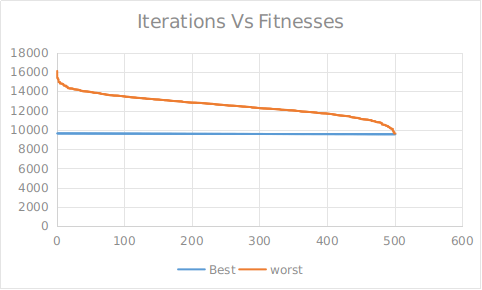
\includegraphics[width=\linewidth]{37.png}
						\captionof{figure}{Schwefel (Experiment \#1)}
					\end{minipage}
					\hfill
					\begin{minipage}{0.6\linewidth}
						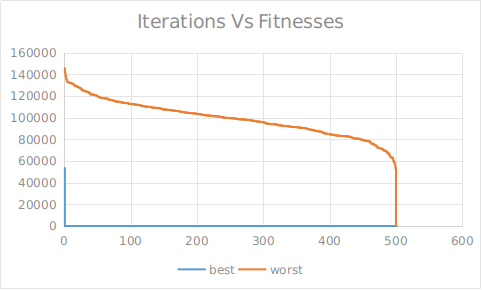
\includegraphics[width=\linewidth]{38.png}
						\captionof{figure}{De Jong 1 (Experiment \#1)}
					\end{minipage}
					\begin{minipage}{0.6\linewidth}
						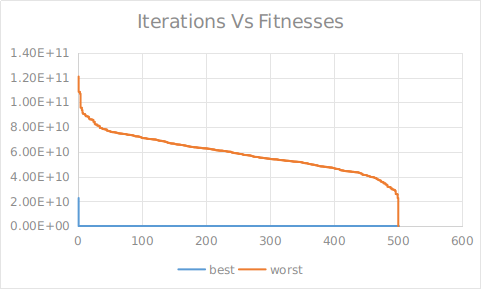
\includegraphics[width=\linewidth]{39.png}
						\captionof{figure}{Rosenbrock (Experiment \#1)}
					\end{minipage}
					\hfill
					\begin{minipage}{0.6\linewidth}
						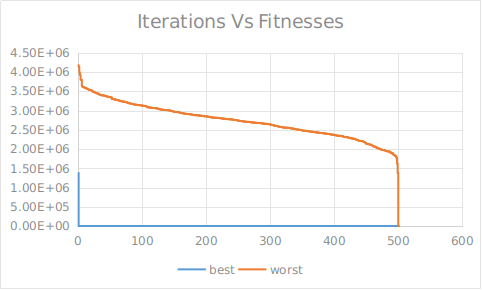
\includegraphics[width=\linewidth]{40.png}
						\captionof{figure}{Rastrigin (Experiment \#1)}
					\end{minipage}
					\begin{minipage}{0.6\linewidth}
						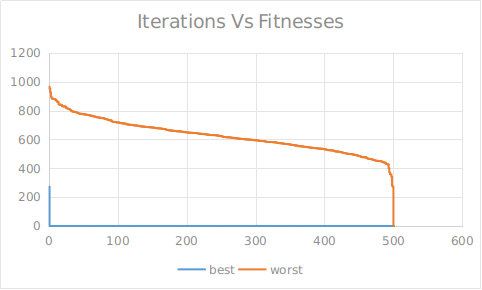
\includegraphics[width=\linewidth]{41.png}
						\captionof{figure}{Griewangk (Experiment \#1)}
					\end{minipage}
					\hfill
					\begin{minipage}{0.6\linewidth}
						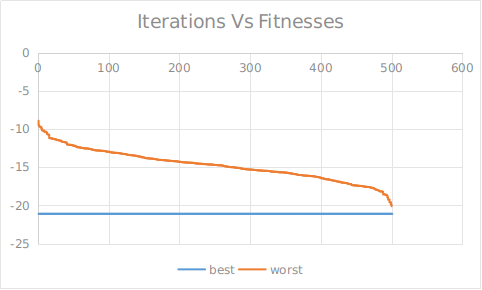
\includegraphics[width=\linewidth]{42.png}
						\captionof{figure}{Sine Envelope (Experiment \#1)}
					\end{minipage}
					\begin{minipage}{0.6\linewidth}
						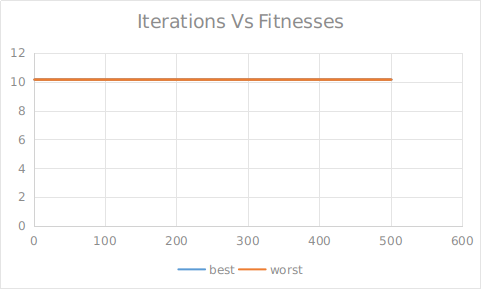
\includegraphics[width=\linewidth]{43.png}
						\captionof{figure}{Stretch V Sine (Experiment \#1)}
					\end{minipage}
					\hfill
					\begin{minipage}{0.6\linewidth}
						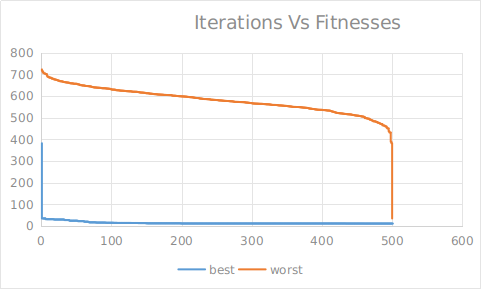
\includegraphics[width=\linewidth]{44.png}
						\captionof{figure}{Ackley One (Experiment \#1)}
					\end{minipage}
					\begin{minipage}{0.6\linewidth}
						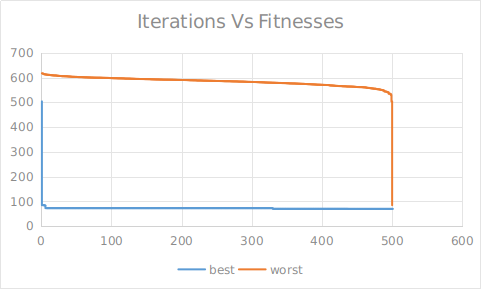
\includegraphics[width=\linewidth]{45.png}
						\captionof{figure}{Ackley Two (Experiment \#1)}
					\end{minipage}
					\hfill
					\begin{minipage}{0.6\linewidth}
						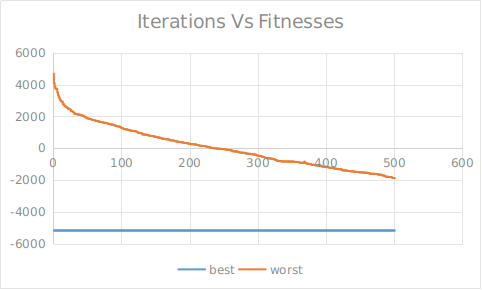
\includegraphics[width=\linewidth]{46.png}
						\captionof{figure}{Egg Holder (Experiment \#1)}
					\end{minipage}
					\begin{minipage}{0.6\linewidth}
						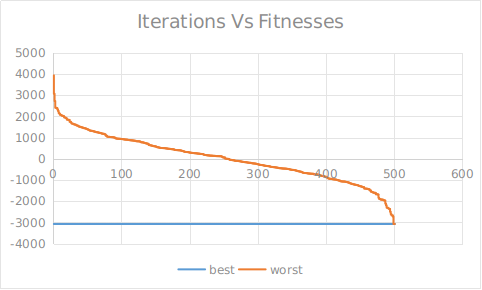
\includegraphics[width=\linewidth]{47.png}
						\captionof{figure}{Rana (Experiment \#1)}
					\end{minipage}
					\hfill
					\begin{minipage}{0.6\linewidth}
						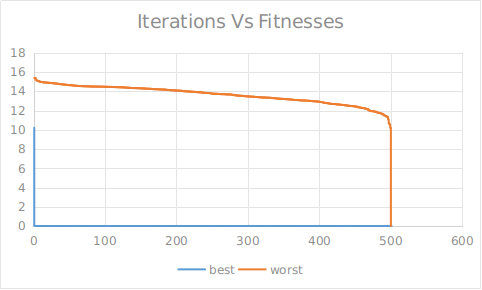
\includegraphics[width=\linewidth]{48.png}
						\captionof{figure}{Pathological (Experiment \#1)}
					\end{minipage}
					\begin{minipage}{0.6\linewidth}
						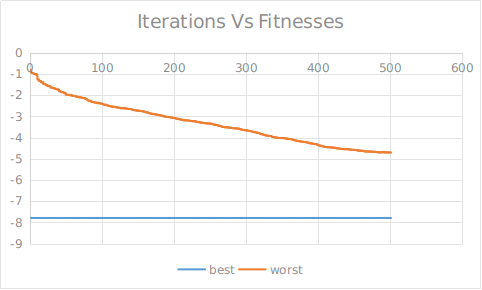
\includegraphics[width=\linewidth]{49.png}
						\captionof{figure}{Michalewicz (Experiment \#1)}
					\end{minipage}
					\hfill
					\begin{minipage}{0.6\linewidth}
						\includegraphics[width=\linewidth]{50.png}
						\captionof{figure}{Masters’ Cosine (Experiment \#1)}
					\end{minipage}
					\begin{minipage}{0.6\linewidth}
						\includegraphics[width=\linewidth]{51.png}
						\captionof{figure}{Quartic (Experiment \#1)}
					\end{minipage}
					\hfill
					\begin{minipage}{0.6\linewidth}
						\includegraphics[width=\linewidth]{52.png}
						\captionof{figure}{Levy (Experiment \#1)}
					\end{minipage}
					\begin{minipage}{0.6\linewidth}
						\includegraphics[width=\linewidth]{53.png}
						\captionof{figure}{Step (Experiment \#1)}
					\end{minipage}
					\hfill
					\begin{minipage}{0.6\linewidth}
						\includegraphics[width=\linewidth]{54.png}
						\captionof{figure}{Alpine (Experiment \#1)}
					\end{minipage}
				\subsubsection{Plots analysis}
				
					When looking at the figures above, we can see that HS improves the quality of the solutions as it goes through iterations. The reason to this improvement is that after each iteration, the pitch of the bad harmonies are adjusted either randomly or using a specific function in order to get them closer the best ones. However, Figures 42, 43, 46, 47, 49 and 50 corresponding to functions Sine Envelope, Stretch V Sine, Egg Holder, Rana, Michalewicz and Master's Cosine respectively also show that HS does not work well for all the functions. In this case, the best solutions remain stable across iterations.
				\newpage
				\subsubsection{Stagnation iterations}
				
				% latex table generated in R 3.5.3 by xtable 1.8-4 package
				% Mon May 20 00:49:11 2019
				\begin{table}[ht]
					\caption{Iteration at which population stagnates (0 means no stagnation observed)}
					\centering
					\scalebox{0.7}{
						\begin{tabular}{lllllllllllllllllll}
							\hline
							& {\textbf{f1}} & {\textbf{f2}} & {\textbf{f3}} & {\textbf{f4}} & {\textbf{f5}} & {\textbf{f6}} & {\textbf{f7}} & {\textbf{f8}} & {\textbf{f9}} & {\textbf{f10}} & {\textbf{f11}} & {\textbf{f12}} & {\textbf{f13}} & {\textbf{f14}} & {\textbf{f15}} & {\textbf{f16}} & {\textbf{f17}} & {\textbf{f18}} \\ 
							\hline
							{\textit{iter 1}} &   0 &   0 &   0 &   0 &   0 &   0 & 500 &   0 &   0 &   0 & 500 &   0 &   0 & 500 &   0 &   0 &   0 &   0 \\ 
							{\textit{iter 2}} &   0 &   0 &   0 &   0 &   0 &   0 & 500 &   0 &   0 &   0 & 500 &   0 &   0 & 500 &   0 &   0 &   0 &   0 \\ 
							{\textit{fiter 3}} &   0 &   0 &   0 &   0 &   0 & 500 & 500 &   0 &   0 &   0 & 500 &   0 &   0 & 500 &   0 &   0 &   0 &   0 \\ 
							{\textit{iter 4}} &   0 &   0 &   0 &   0 &   0 &   0 & 500 &   0 &   0 &   0 & 500 &   0 &   0 & 500 &   0 &   0 &   0 &   0 \\ 
							{\textit{iter 5}} &   0 &   0 &   0 &   0 &   0 &   0 & 500 &   0 &   0 &   0 & 500 &   0 &   0 & 500 &   0 &   0 &   0 &   0 \\ 
							{\textit{iter 6}} &   0 &   0 &   0 &   0 &   0 & 500 & 500 &   0 &   0 &   0 & 500 &   0 &   0 & 500 &   0 &   0 &   0 &   0 \\ 
							{\textit{iter 7}} &   0 &   0 &   0 &   0 &   0 &   0 & 500 &   0 &   0 &   0 & 500 &   0 &   0 & 500 &   0 &   0 &   0 &   0 \\ 
							{\textit{iter 8}} &   0 &   0 &   0 &   0 &   0 &   0 & 500 &   0 &   0 &   0 & 500 &   0 &   0 & 500 &   0 &   0 &   0 &   0 \\ 
							{\textit{iter 9}} &   0 &   0 &   0 &   0 &   0 &   0 & 500 &   0 &   0 &   0 & 500 &   0 &   0 & 500 &   0 &   0 &   0 &   0 \\ 
							{\textit{iter 10}} &   0 &   0 &   0 &   0 &   0 &   0 & 500 &   0 &   0 &   0 & 500 &   0 &   0 & 500 &   0 &   0 &   0 &   0 \\ 
							{\textit{iter 11}} &   0 &   0 &   0 &   0 &   0 &   0 & 500 &   0 &   0 &   0 & 500 &   0 &   0 & 500 &   0 &   0 &   0 &   0 \\ 
							{\textit{iter 12}} &   0 &   0 &   0 &   0 &   0 &   0 & 500 &   0 &   0 &   0 & 500 &   0 &   0 & 500 &   0 &   0 &   0 &   0 \\ 
							{\textit{iter 13}} &   0 &   0 &   0 &   0 &   0 &   0 & 500 &   0 &   0 &   0 & 500 &   0 &   0 & 500 &   0 &   0 &   0 &   0 \\ 
							{\textit{iter 14}} &   0 &   0 &   0 &   0 &   0 &   0 & 500 &   0 &   0 &   0 & 500 &   0 &   0 & 500 &   0 &   0 &   0 &   0 \\ 
							{\textit{iter 15}} &   0 &   0 &   0 &   0 &   0 &   0 & 500 &   0 &   0 &   0 & 500 &   0 &   0 & 500 &   0 &   0 &   0 &   0 \\ 
							{\textit{iter 16}} &   0 &   0 &   0 &   0 &   0 &   0 & 500 &   0 &   0 &   0 & 500 &   0 &   0 & 500 &   0 &   0 &   0 &   0 \\ 
							{\textit{iter 17}} &   0 &   0 &   0 &   0 &   0 &   0 & 500 &   0 &   0 &   0 & 500 &   0 &   0 & 500 &   0 &   0 &   0 &   0 \\ 
							{\textit{iter 18}} &   0 &   0 &   0 &   0 &   0 &   0 & 500 &   0 &   0 &   0 & 500 &   0 &   0 & 500 &   0 &   0 &   0 &   0 \\ 
							{\textit{iter 19}} &   0 &   0 &   0 &   0 &   0 & 500 & 500 &   0 &   0 &   0 & 500 &   0 &   0 & 500 &   0 &   0 &   0 &   0 \\ 
							{\textit{iter 20}} &   0 &   0 &   0 &   0 &   0 &   0 & 500 &   0 &   0 &   0 & 500 &   0 &   0 & 500 &   0 &   0 &   0 &   0 \\ 
							{\textit{iter 21}} &   0 &   0 &   0 &   0 &   0 & 500 & 500 &   0 &   0 &   0 & 500 &   0 &   0 & 500 &   0 &   0 &   0 &   0 \\ 
							{\textit{iter 22}} &   0 &   0 &   0 &   0 &   0 &   0 & 500 &   0 &   0 &   0 & 500 &   0 &   0 & 500 &   0 &   0 &   0 &   0 \\ 
							{\textit{iter 23}} &   0 &   0 &   0 &   0 &   0 &   0 & 500 &   0 &   0 &   0 & 500 &   0 &   0 & 500 &   0 &   0 &   0 &   0 \\ 
							{\textit{iter 24}} &   0 &   0 &   0 &   0 &   0 & 500 & 500 &   0 &   0 &   0 & 500 &   0 &   0 & 500 &   0 &   0 &   0 &   0 \\ 
							{\textit{iter 25}} &   0 &   0 &   0 &   0 &   0 &   0 & 500 &   0 &   0 &   0 & 500 &   0 &   0 & 500 &   0 &   0 &   0 &   0 \\ 
							{\textit{iter 26}} &   0 &   0 &   0 &   0 &   0 &   0 & 500 &   0 &   0 &   0 & 500 &   0 &   0 & 500 &   0 &   0 &   0 &   0 \\ 
							{\textit{iter 27}} &   0 &   0 &   0 &   0 &   0 &   0 & 500 &   0 &   0 &   0 & 500 &   0 &   0 & 500 &   0 &   0 &   0 &   0 \\ 
							{\textit{iter 28}} &   0 &   0 &   0 &   0 &   0 &   0 & 500 &   0 &   0 &   0 & 500 &   0 &   0 & 500 &   0 &   0 &   0 &   0 \\ 
							{\textit{iter 29}} &   0 &   0 &   0 &   0 &   0 &   0 & 500 &   0 &   0 &   0 & 500 &   0 &   0 & 500 &   0 &   0 &   0 &   0 \\ 
							{\textit{iter 30}} &   0 &   0 &   0 &   0 &   0 &   0 & 500 &   0 &   0 &   0 & 500 &   0 &   0 & 500 &   0 &   0 &   0 &   0 \\ 
							\hline
						\end{tabular}
					}
				\end{table}
					
					
		\section{Conclusion}
			After implementing, experimenting and analyzing three different instances of the particle swarm intelligence algorithms, it can be determined that particle swarm intelligence algorithms not only are easier to implement than evolutionary algorithms but also produce better results even though they might take more time to process in some cases (FA). However, analysis of the results of PSO, FA and HS showed that none of them works for functions such as Sine Envelope, Stretch V Sine, Egg Holder, Rana, Michalewicz and Master's Cosine
			
\end{document}